% SC3020 --- Chapter 6: Association Analysis (0->100 ground-up)
\chapter{Association Analysis}
\label{ch:association}

\begin{quote}
\emph{``People who bought this also bought \dots''} Association mining finds co-occurrence rules that drive recommendations, shelf placement, and fraud detection.
\end{quote}

\noindent\fbox{\parbox{\dimexpr\linewidth-2\fboxsep-2\fboxrule}{%
\textbf{From zero: no market-basket assumed.} We start from a receipt, define itemsets, support, confidence and lift, then formalise Apriori and FP-growth from intuition to complexity. Pictures precede enumeration.}}
\vspace{0.4em}

\section*{Learning Outcomes}
After this chapter you will be able to:
\begin{enumerate}[label=(L\arabic*)]
    \item define support, confidence, and lift and interpret their trade-offs;
    \item enumerate frequent itemsets via the Apriori principle and pruning;
    \item build and mine an FP-tree (FP-growth) without candidate generation;
    \item evaluate rules (lift $>$ 1, redundancy, statistical significance);
    \item apply association mining to a sparse transaction matrix in Python.
\end{enumerate}

% ============================================================
\section{Rules and Interestingness}
\label{sec:rules}
\paragraph{Intuition.} A supermarket receipt is a basket $\{ \text{bread}, \text{butter}, \text{milk}\}$. The rule $\{ \text{bread},\text{butter}\}\Rightarrow\{\text{milk}\}$ says ``if a basket has bread and butter, it also tends to have milk.'' Usefulness depends on frequency ($\approx$ many baskets?) and reliability ($\approx$ when antecedent occurs, how often does consequent follow?) and strength beyond chance.

\paragraph{Formal measures.} Let $\mathcal{I}$ be items, transaction $T\subseteq\mathcal{I}$, database $\mathcal{D}=\{T_1,\dots,T_N\}$. Itemset $X$ has \emph{support}
\begin{equation}
\text{supp}(X)=\frac{|\{T\in\mathcal{D}:X\subseteq T\}|}{N}=P(X),
\end{equation}
the empirical joint probability. Rule $X\Rightarrow Y$ ($X\cap Y=\emptyset$) has
\begin{equation}
\text{conf}(X\Rightarrow Y)=\frac{\text{supp}(X\cup Y)}{\text{supp}(X)}=P(Y\mid X),\qquad
\text{lift}(X\Rightarrow Y)=\frac{\text{conf}(X\Rightarrow Y)}{\text{supp}(Y)}=\frac{P(X\cup Y)}{P(X)P(Y)}.
\end{equation}
$\text{lift}=1$ means independence; $>1$ positive association; $<1$ negative. Support filters rare noise; confidence measures predictive power; lift corrects for popularity of $Y$ (a high-confidence rule can have lift $\approx1$ if $Y$ is ubiquitous).

\begin{figure}[h]\centering
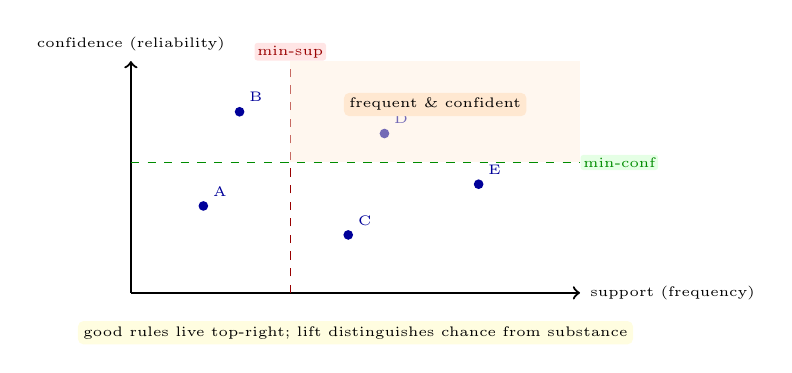
\begin{tikzpicture}[scale=0.92, every node/.style={font=\scriptsize}]
\draw[->, thick] (0,0)--(6.2,0) node[right, font=\tiny] {support (frequency)};
\draw[->, thick] (0,0)--(0,3.2) node[above, font=\tiny] {confidence (reliability)};
% scatter of rules
\foreach \x/\y/\lbl in {1.0/1.2/A, 1.5/2.5/B, 3.0/0.8/C, 3.5/2.2/D, 4.8/1.5/E} {
  \fill[blue!60!black] (\x,\y) circle (1.9pt) node[above right, font=\tiny] {\lbl};
}
% thresholds
\draw[dashed, red!60!black] (2.2,0)--(2.2,3.2) node[above, font=\tiny, fill=red!10, rounded corners=1pt, inner sep=1pt] {min-sup};
\draw[dashed, green!55!black] (0,1.8)--(6.2,1.8) node[right, font=\tiny, fill=green!10, rounded corners=1pt, inner sep=1pt] {min-conf};
\fill[orange!14, opacity=0.45] (2.2,1.8) rectangle (6.2,3.2);
\node[font=\tiny, fill=orange!18, rounded corners=2pt, inner sep=2pt] at (4.2,2.6) {frequent \& confident};
\node[font=\tiny, fill=yellow!12, rounded corners=2pt, inner sep=2pt] at (3.1,-0.55) {good rules live top-right; lift distinguishes chance from substance};
\end{tikzpicture}
\caption{Rule space. Each point is a rule $X\Rightarrow Y$. Thresholds on support and confidence select candidates; lift then ranks by interestingness beyond baseline.}
\label{fig:rule-space}
\end{figure}

% ============================================================
\section{Apriori: Level-Wise Search with Pruning}
\label{sec:apriori}
\paragraph{Intuition.} Brute-forcing all $2^{|\mathcal{I}|}$ itemsets is impossible. Apriori exploits monotonicity: if $\{a,b\}$ is infrequent, any superset $\{a,b,c\}$ is also infrequent --- prune the whole subtree.

\paragraph{Principle and algorithm.} \emph{Apriori property}: all non-empty subsets of a frequent itemset are frequent; contrapositive gives downward closure for pruning. Algorithm (BFS level-wise): $L_1=\{ \text{frequent 1-itemsets}\}$; for $k=2,\dots$ generate candidates $C_k$ by joining $L_{k-1}$ (pairs sharing $k-2$ items), prune any $c\in C_k$ with an infrequent $(k-1)$-subset, scan $\mathcal{D}$ to count support, keep $L_k=\{c\in C_k:\text{supp}(c)\ge\text{min-sup}\}$. Stop when $L_k=\emptyset$. Then generate rules $X\Rightarrow Y$ with $X\cup Y\in\bigcup_k L_k$ and $\text{conf}\ge\text{min-conf}$. Complexity dominated by scans and candidate blow-up on dense data.

\begin{figure}[h]\centering
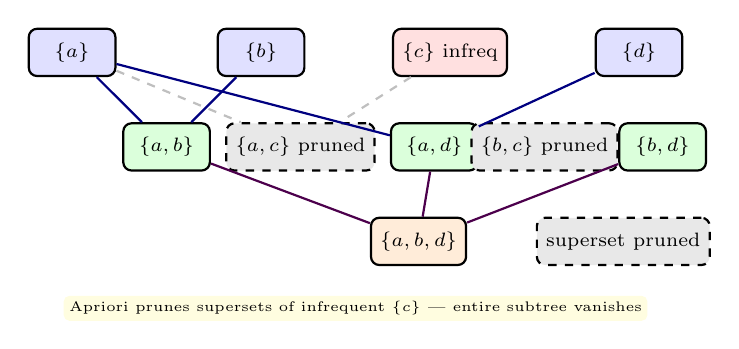
\begin{tikzpicture}[every node/.style={font=\scriptsize},
  n/.style={draw, thick, rounded corners=3pt, align=center, minimum width=1.1cm, minimum height=0.6cm}]
% lattice level 1
\node[n, fill=blue!12] (a) at (0,2.4) {$\{a\}$};
\node[n, fill=blue!12] (b) at (2.4,2.4) {$\{b\}$};
\node[n, fill=red!12] (c) at (4.8,2.4) {$\{c\}$ infreq};
\node[n, fill=blue!12] (d) at (7.2,2.4) {$\{d\}$};
% level 2
\node[n, fill=green!14] (ab) at (1.2,1.2) {$\{a,b\}$};
\node[n, fill=gray!18, dashed] (ac) at (2.9,1.2) {$\{a,c\}$ pruned};
\node[n, fill=green!14] (ad) at (4.6,1.2) {$\{a,d\}$};
\node[n, fill=gray!18, dashed] (bc) at (6.0,1.2) {$\{b,c\}$ pruned};
\node[n, fill=green!14] (bd) at (7.5,1.2) {$\{b,d\}$};
% level 3
\node[n, fill=orange!15] (abd) at (4.4,0.0) {$\{a,b,d\}$};
\node[n, fill=gray!18, dashed] (abcd) at (7.0,0.0) {superset pruned};
% edges
\draw[thick, blue!50!black] (a)--(ab); \draw[thick, blue!50!black] (b)--(ab);
\draw[thick, gray!50, dashed] (a)--(ac); \draw[thick, gray!50, dashed] (c)--(ac);
\draw[thick, blue!50!black] (a)--(ad); \draw[thick, blue!50!black] (d)--(ad);
\draw[thick, violet!60!black] (ab)--(abd); \draw[thick, violet!60!black] (ad)--(abd); \draw[thick, violet!60!black] (bd)--(abd);
\node[font=\tiny, fill=yellow!12, rounded corners=2pt, inner sep=2pt] at (3.6,-0.85) {Apriori prunes supersets of infrequent $\{c\}$ --- entire subtree vanishes};
\end{tikzpicture}
\caption{Lattice view of Apriori with min-sup pruning. Gray dashed nodes are never counted because a subset is already infrequent.}
\label{fig:apriori-lattice}
\end{figure}

% ============================================================
\section{FP-Growth: Compress and Mine Without Candidates}
\label{sec:fpgrowth}
\paragraph{Intuition.} Instead of generating candidates, compress $\mathcal{D}$ into a prefix tree keyed by frequency order. Frequent patterns share prefixes, so the tree is compact; mining recursively extracts patterns by building conditional trees.

\paragraph{Steps.} (1) Scan $\mathcal{D}$: count support of 1-itemsets, keep frequent, sort each transaction descending by support. (2) Insert transactions into the \emph{FP-tree}: root $\to$ branch per item, counters along path. Header table links same items. (3) Mine: for each item $i$ (ascending support), collect its \emph{conditional pattern base} (prefix paths co-occurring with $i$), build conditional FP-tree, recurse. Each conditional tree is smaller; recursion enumerates all frequent patterns without candidate generation. FP-growth excels on dense/compressed data; worst-case still exponential (output size).

\begin{figure}[h]\centering
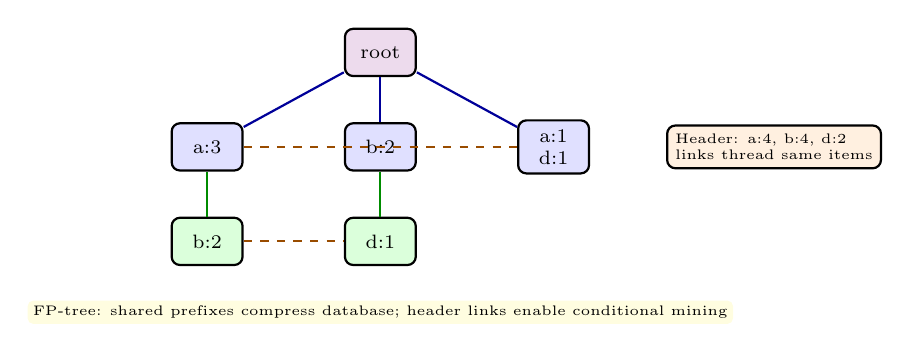
\begin{tikzpicture}[every node/.style={font=\scriptsize}, level distance=10mm, sibling distance=14mm,
  f/.style={draw, thick, rounded corners=3pt, fill=blue!12, minimum width=0.9cm, minimum height=0.6cm, align=center}]
\node[f, fill=violet!14] (r) at (0,0) {root};
\node[f] (a) at (-2.2,-1.2) {a:3} child[missing];
\node[f] (b) at (0,-1.2) {b:2};
\node[f] (ad) at (2.2,-1.2) {a:1\\d:1};
\draw[thick, blue!60!black] (r)--(a); \draw[thick, blue!60!black] (r)--(b); \draw[thick, blue!60!black] (r)--(ad);
\node[f, fill=green!14] (ab) at (-2.2,-2.4) {b:2};
\node[f, fill=green!14] (bd) at (0,-2.4) {d:1};
\draw[thick, green!55!black] (a)--(ab); \draw[thick, green!55!black] (b)--(bd);
% header
\node[draw, thick, fill=orange!12, rounded corners=3pt, align=left, inner sep=3pt, font=\tiny] (h) at (5.0,-1.2) {Header: a:4, b:4, d:2\\links thread same items};
\draw[dashed, orange!60!black, thick] (a) -- (ad);
\draw[dashed, orange!60!black, thick] (ab) -- (bd);
\node[font=\tiny, fill=yellow!12, rounded corners=2pt, inner sep=2pt] at (0,-3.3) {FP-tree: shared prefixes compress database; header links enable conditional mining};
\end{tikzpicture}
\caption{Schematic FP-tree for transactions with order $a>b>d$. Counts on nodes are supports along the prefix path; header links (dashed) chain identical items.}
\label{fig:fptree}
\end{figure}

\begin{lstlisting}[language=Python, caption={From transactions to rules: Apriori via mlxtend.}, label={lst:apriori}]
import pandas as pd
from mlxtend.frequent_patterns import apriori, association_rules

# Toy transactions as one-hot DataFrame
data = [{"bread":1,"butter":1,"milk":1},
        {"bread":1,"butter":1,"milk":0},
        {"bread":0,"butter":1,"milk":1},
        {"bread":1,"butter":0,"milk":1},
        {"bread":1,"butter":1,"milk":1}]
df = pd.DataFrame(data).astype(bool)

freq = apriori(df, min_support=0.4, use_colnames=True)
rules = association_rules(freq, metric="confidence", min_threshold=0.6)
rules["lift"] = rules["confidence"] / rules["consequent support"]
print(freq.sort_values("support", ascending=False))
print(rules[["antecedents","consequents","support","confidence","lift"]])
\end{lstlisting}

\begin{lstlisting}[language=Python, caption={Computing lift manually and filtering spurious rules.}, label={lst:lift}]
# Add statistical lens: Fisher exact test for rule significance
from scipy.stats import fisher_exact
import numpy as np
# contingency for {bread,butter} => {milk}
#            milk  not-milk
#  {b,bt}     a=2     b=1
# not        c=1     d=1
a,b,c,d = 2,1,1,1
odds, p = fisher_exact([[a,b],[c,d]])
print(f"lift={a/(a+b) / ((a+c)/5):.2f}, Fisher p={p:.3f} (small p = significant)")
# In practice: correct for multiple testing (Bonferroni / FDR)
\end{lstlisting}

% ============================================================
\section{Judging and Using Rules}
\label{sec:using-rules}
High support $+$ high confidence is not enough: a rule $\{ \text{milk}\}\Rightarrow\{ \text{bread}\}$ may be confident only because bread is common. Require lift $>1.2$ or leverage $\text{supp}(X\cup Y)-\text{supp}(X)\text{supp}(Y)>0$. Remove \emph{redundant} rules where a more general antecedent has similar confidence; consider \emph{closed} and \emph{maximal} itemsets for compact representation. Validate causally: association $\neq$ causation (beer and nappies both peak on Fridays --- common cause, not one causing the other).

% ============================================================
% ============================================================
\section{Compact Representations and Sequential Patterns}
\label{sec:compact}
\paragraph{Closed and maximal.} An itemset $X$ is \emph{closed} if no proper superset has the same support; \emph{maximal} if no superset is frequent. Closed sets preserve exact supports with far fewer patterns; maximal sets are smaller still but lose exact support. Use closed when reporting to humans.

\paragraph{Sequential patterns.} Transactions ordered by time become sequences. Rule examples: $\langle\text{buy phone}\rangle \to \langle\text{buy case}\rangle$ within 7 days. Algorithms like GSP and PrefixSpan generalise Apriori to sequences where order matters and gaps are allowed.

\paragraph{Practical filters.} Beyond lift, use \emph{conviction} $\frac{1-\text{supp}(Y)}{1-\text{conf}}$ ($\infty$ when rule never violates), \emph{all-confidence} for hypercliques, and statistical tests with multiple-testing correction. Visualise top rules with grouped matrix or graph plots where nodes are items and edges are rules.

\begin{lstlisting}[language=Python, caption={Closed itemsets intuition: filtering redundant patterns.}, label={lst:closed}]
# After apriori(freq) -> keep only closed
freq["len"] = freq["itemsets"].apply(len)
# closed if no superset with same support (naive O(m2) check, OK for demo)
is_closed = []
for i, row in freq.iterrows():
    supers = freq[freq["itemsets"].apply(lambda s: row["itemsets"] < s)]
    closed = not any(supers["support"] == row["support"])
    is_closed.append(closed)
print(freq[is_closed].sort_values("support", ascending=False))
\end{lstlisting}

% ============================================================
% ============================================================
\section{From Rules to Recommendations}
\label{sec:recommend}
\paragraph{Recommender link.} Association rules power \emph{market-basket recommenders}: if cart contains $X$, recommend top-$k$ consequents $Y$ ranked by lift $\times$ support or by confidence with a support floor. Add recency and business constraints (margin, inventory).

\paragraph{Evaluation.} Offline: hit-rate and mean average precision on held-out baskets. Online: A/B test click-through and revenue. A rule can be statistically significant yet commercially useless if $Y$ is already in the cart or trivially popular.

\paragraph{Scaling.} On 10M baskets, Apriori floods. FP-growth with partitioning (or Spark's FPGrowth) scales horizontally; sampling with error bounds (\`a la Toivonen) gives fast approximate frequent sets.

% ============================================================
\section{Chapter Notes}
Agrawal, Imielinski \& Swami (1993) introduced association rules; Apriori is Agrawal \& Srikant (1994); FP-growth is Han et al. (2000) --- now the default for sparse large data. For sequential patterns see PrefixSpan; for recommender context see Ch.~8.

% ============================================================
\section{Exercises}
\begin{enumerate}[label=E6.\arabic*, leftmargin=*, itemsep=0.6em]
    \item \textbf{Measures.} Transactions: 100 total; $\{a\}$ in 40, $\{b\}$ in 50, $\{a,b\}$ in 20. Compute support, confidence, and lift for $\{a\}\Rightarrow\{b\}$ and $\{b\}\Rightarrow\{a\}$. Is the association positive?
    \item \textbf{Apriori trace.} Items $\{1,2,3,4\}$, transactions $\{\{1,2,3\},\{1,2\},\{1,3\},\{2,3,4\}\}$, min-sup $=0.5$ ($\ge2$ transactions). List $L_1,L_2,L_3$ and pruned candidates at each level.
    \item \textbf{FP-tree.} Build an FP-tree for transactions $\{\{a,b\},\{b,c\},\{a,b,c\},\{a,c\}\}$ with order by global frequency. Show header table and the conditional base for item $c$.
    \item \textbf{Lift vs.\ confidence.} Give a dataset where a rule has confidence $0.9$ but lift $\approx1$. Explain why lift matters for recommendation and name one alternative measure (leverage, conviction).
    \item \textbf{Multiple testing.} Why does mining thousands of rules inflate false positives? Propose a correction (Bonferroni or FDR) and discuss its trade-off.
\end{enumerate}
% End of Chapter 6
